\documentclass[aspectratio=169]{beamer}

\usepackage{amssymb,amsmath}
\usepackage{graphicx}
\usepackage{url}
\usepackage{color}
\usepackage{pagenote}[continuous,page]
\usepackage{relsize}		% For \smaller
\usepackage{url}			% For \url
\usepackage{epstopdf}	% Included EPS files automatically converted to PDF to include with pdflatex

%For MindMaps
% \usepackage{tikz}%
% \usetikzlibrary{mindmap,trees,arrows}%

%%% Color Definitions %%%%%%%%%%%%%%%%%%%%%%%%%%%%%%%%%%%%%%%%%%%%%%%%%%%%%%%%%
%\definecolor{bordercol}{RGB}{40,40,40}
%\definecolor{headercol1}{RGB}{186,215,230}
%\definecolor{headercol2}{RGB}{80,80,80}
%\definecolor{headerfontcol}{RGB}{0,0,0}
%\definecolor{boxcolor}{RGB}{186,215,230}

%%% Save space in lists. Use this after the opening of the list %%%%%%%%%%%%%%%%
%\newcommand{\compresslist}{
%	\setlength{\itemsep}{1pt}
%	\setlength{\parskip}{0pt}
%	\setlength{\parsep}{0pt}
%}

%\setbeameroption{show notes on top}

% You should run 'pdflatex' TWICE, because of TOC issues.

% Rename this file.  A common temptation for first-time slide makers
% is to name it something like ``my_talk.tex'' or
% ``john_doe_talk.tex'' or even ``discrete_math_seminar_talk.tex''.
% You really won't like any of these titles the second time you give a
% talk.  Try naming your tex file something more descriptive, like
% ``riemann_hypothesis_short_proof_talk.tex''.  Even better (in case
% you recycle 99% of a talk, but still want to change a little, and
% retain copies of each), how about
% ``riemann_hypothesis_short_proof_MIT-Colloquium.2000-01-01.tex''?

\mode<presentation>
{
  \usetheme{CambridgeUS}		% bem bacana - menu superior
  \usecolortheme{default}		% branco, azul clarinho
  \useoutertheme{default}
  \useinnertheme{circles}
  \setbeamercovered{invisible}
}

\beamertemplatenavigationsymbolsempty

%% Better looking blocks
\setbeamercolor{block title alerted}{use=structure,fg=black,bg=red!80!black}
\setbeamercolor{block body alerted}{use=structure,fg=black,bg=white!90!black}

\setbeamercolor{block title}{use=structure,fg=black,bg=blue!60!white}
\setbeamercolor{block body}{use=structure,fg=black,bg=white!90!black}

\usepackage[english]{babel}
\usepackage[latin1]{inputenc}
\usepackage{subfigure}

\usepackage{times}
\usepackage[T1]{fontenc}

%% makes the ppagenote command for figure references at the end.
\makepagenote
\renewcommand{\notenumintext}[1]{}
\newcommand{\ppagenote}[1]{\pagenote[Page \insertframenumber]{#1}}


\title[GB13624]{GB13624 - Maths for Computer Science}
\subtitle[]{Lecture 1 -- Introduction to Proofs}
\author[Claus Aranha]{Claus Aranha\\{\footnotesize caranha@cs.tsukuba.ac.jp}}
\institute[COINS]{College of Information Science}
\date[2024-10-02]{2024-10-02\\{\tiny Last updated \today}}

\begin{document}

\begin{frame}
  \maketitle
\end{frame}

\section{Introduction}

\begin{frame}{Lecture 1 -- Outline}
  In this lecture, we introduce the concept of {\bf mathematical proofs}:\bigskip

  \begin{itemize}
    \item {\bf Section 1:} What are proofs, and why we need them;
    \item {\bf Section 2:} Basic proof methods;
    \item {\bf Section 3:} The Well Ordering Principle (WOP);\\
    (an important proof method)
    \item {\bf Section 4:} Logical formulas and satisfiability;
  \end{itemize}


  \bigskip
  \begin{block}{}
  This lecture covers the textbook's chapters 1, 2 and 3.
  \end{block}
\end{frame}

\section{Introduction to Proofs}

\frame{
{Part 1: Introduction to Proofs.}

\tableofcontents[currentsection,hideallsubsections, firstsection=2, sections={2-5}]
}

\subsection{What is a Proof?}

\begin{frame}{What is a proof?}

  Some concepts are easy to understand, but not easy to show that they are true.\bigskip

  \begin{columns}
    \column{0.3\textwidth}
      \centering
      \includegraphics[width=.5\textwidth]{../img/triangle_rect}
    \column{0.7\textwidth}
      \begin{itemize}
        \item Pythagoras Theorem:
        \begin{equation*}
          a^2+b^2=c^2
        \end{equation*}
        \item It is easy to show this is true for {\bf any one triangle}.
        \item But how do you show it is is true for {\bf all} triangles?
      \end{itemize}
  \end{columns}
  \bigskip

  The proof of the Pythagoras theorem is {not obvious}: there are more than 100 different proofs!
\end{frame}

\begin{frame}{What is a proof?}{One Pythagoras Proof}

  \begin{columns}[T]
    \column{0.7\textwidth}
      \begin{itemize}
        \item {\bf Proof}: by geometric construction
        \item Arrange four identical triangles;
        \item Show that internal angles are right;
        \item Internal square area: $c^2$
        \item External square area: $(a+b)^2$
        \item $(a+b)^2 = c^2 + 4(\text{area triangle})$
        \item $(a+b)^2 = c^2 + 4(\frac{ab}{2})$
        \item $a^2 + 2ab + b^2 = c^2 + 2ab$
        \item $a^2 + b^2 = c^2$ \hfill $\blacksquare$
      \end{itemize}
    \column{0.3\textwidth}
      \includegraphics[width=\textwidth]{../img/triangle_pytagoras}
  \end{columns}
  \bigskip

  {\bf Remember:} There are many other possible proofs. (Beautiful proofs, short proofs, wrong proofs, etc.)
\end{frame}

\begin{frame}{False Proofs}{Infinite Chocolate!}
  \begin{center}
    \includegraphics[width=.9\textwidth]{../img/false_proof}
  \end{center}
  \begin{itemize}
    \item What is wrong with the proof above?
    \item \alert{Be careful!} A false proof can have many correct steps, and {\bf only one} impossible step.
  \end{itemize}

  \begin{block}{}
    We can use proofs to show that something is {\bf incorrect} as well!
  \end{block}
\end{frame}

\subsection{Proofs and Computer Science}

\begin{frame}{Proofs and Computer Science}{Why are proofs important for Computer Science?}

  \begin{itemize}
    \item We don't use proofs only for mathematical equations.
    \item We can use proofs to {\bf show that a program is correct}. (or incorrect)
    \vfill

    \item Example cases:
    \begin{itemize}
    \item Use proofs to show that the result of a program is correct for any input;
    \item Use proofs to show that one type of input will cause a bug in the program;
    \item Use proofs to show that a program finishes in $N$ steps;
    \end{itemize}
  \end{itemize}
\end{frame}

\begin{frame}[fragile]{Proofs and Computer Science}{Example:}
  \begin{itemize}
    \item Is the program below correct or incorrect?
    \item Can you show by using a proof?
  \end{itemize}
  \bigskip

\begin{verbatim}
int triangle_type(int a, int b, int c)
  // a, b, c are the length of the sides of a triangle;
  if (a == b)
    if (b == c)
      return "all sides are equal";
    else
      return "two sides are equal";
  else if (b == c)
    return "two sides are equal";
  else
    return "all sides are different";
\end{verbatim}
\end{frame}

\begin{frame}{Next Part:}
  Proof Techniques: How do we prove something?
\end{frame}

\section{Proof Methods}

\frame{{Part 2: Proof Methods}

\tableofcontents[currentsection,hideallsubsections, firstsection=2, sections={2-4}]}

\subsection{Inference Rules}

\begin{frame}{Inference Rules}{}
  Inference (or logic deductions) are used to prove new propositions by using propositions that have been proposed before.
  \bigskip

  We normally write an inference as follows:

  \[
  \frac{P, Q, R}{X}
  \]

  This means "propositions P, Q, R are true, meaning that proposition X is true".\bigskip

  \structure{Inference Rules} are inferences that are particularly useful to build proofs. Let's see a few:
\end{frame}

\begin{frame}{Inference Rules}{Modus Ponens}
  The \emph{Modus Ponens} inference rule is:
  \[
  \frac{P, P\implies Q}{Q}
  \]
  If P is true, and P implies Q is true, then Q is true.\bigskip

  A few other related inference rules:
  \[
  \frac{P \implies Q, Q \implies R}{P \implies R},
  \frac{not(P) \implies not(Q)}{Q \implies P}
  \]

  So one way to prove a proposition is to {\bf start with propositions that you know are true} and {\bf use inference rules to reach the proposition you want to prove}.
\end{frame}

\subsection{Proving Implications}

\begin{frame}{Proving an Implication}{Direct Proof}
  The \emph{Modus Ponens} rule says that:
  \[
  \frac{P, P\implies Q}{Q}
  \]
  To prove $Q$, we have to prove that $P$, and that {\bf $P$ implies $Q$}.\bigskip

  We can prove an implication directly, by assuming $P$ is true, and showing that $Q$ must be true, step by step.\bigskip
\end{frame}

\begin{frame}{Proving an Implication}{Direct Proof}
{\bf Theorem:} If $0 \leq x \leq 2$, then $-x^3 + 4x + 1 > 0$\bigskip

\begin{proof}
\begin{itemize}
  \item Let's assume $0 \leq x \leq 2$
  \item We can rewrite $-x^3 + 4x$ as $x(2-x)(2+x)$
  \item If $0 \leq x \leq 2$, then $x$, $(2-x)$, $(2+x)$ are all non-negative.
  \item $x(2-x)(2+x) \geq 0$
  \item $x(2-x)(2+x) + 1 > 0$
  \item $-x^3 + 4x + 1 > 0$
\end{itemize}
\end{proof}

\end{frame}

\begin{frame}{Proving an Implication}{Contrapositive}
  Another way to prove an implication is to "prove the contrapositive". This means using the following inference rule:

  \[
    \frac{\text{NOT}(Q) \implies \text{NOT}(P)}{P \implies Q}
  \]

  So if we show that when Q is false, then P is always false, it is equivalent to show that when P is true, then Q is always true.
\end{frame}

\begin{frame}{Proving an Implication}{Contrapositive}
  {\bf Theorem:} if $r$ is irrational, then $\sqrt{r}$ is also irrational.

  \begin{proof}
    We prove the contrapositive: If $\sqrt{r}$ is rational, then $r$ is also rational.
    \begin{itemize}
      \item If $\sqrt{r}$ is rational, then $\sqrt{r}=\frac{m}{n}$.
      \item $m$ and $n$ are integers (definition of rational numbers)
      \item Square both sides: $r = \frac{m^2}{n^2}$.
      \item $m^2$ and $n^2$ are also integers, so $r$ is rational.
    \end{itemize}
  \end{proof}
\end{frame}



\begin{frame}{Proving "If and only If"}
  Remember that "If and only If" can be defined as:
  \[
  \frac{P\implies Q, Q \implies P}{P\iff Q}
  \]

  So to prove $P\iff Q$, we can first prove the implication from $P$ to $Q$, and then prove the implication from $Q$ to $P$.\bigskip

  This is useful to show equivalence between two mathematical statements.
\end{frame}


\subsection{Proof by Cases}

\begin{frame}[fragile]{Proof By Cases}{Example}

  Let's say you are refactoring code, and you want to profe that the two code samples below are equivalent. How would you do it?
  \vfill

  \begin{block}{Code 1}
\begin{verbatim}
If (X > 0 OR (X <= 0 AND Y > 100))
  print("Hello!")
\end{verbatim}
  \end{block}
  \begin{block}{Code 2}
\begin{verbatim}
If (X > 0 OR Y > 100)
  print("Hello!")
\end{verbatim}
  \end{block}
\end{frame}

\begin{frame}{Proof By Cases}{Definition}
  \structure{Proof By Cases}, is a proof technique that uses the idea of "divide and conquer".\vfill

  You break one complicated problem into easier, smaller sub-problems.
  \vfill

  \alert{Important!} When you create the cases, make sure that all possible cases are covered!
\end{frame}

\begin{frame}{Example: Friends and Strangers}

  {\bf Theorem:} In a group of 6 people, where {\bf every pair} is either a friend or a stranger, then we {\bf always} have at least a set of \structure{3 mutual friends} or a set of \alert{3 mutual strangers}.

  \begin{center}
    \includegraphics[width=0.6\textwidth]{../img/friends_and_strangers}
  \end{center}
  \pagenote{Friends or Strangers Image from "Math for Computer Science" MIT-OCW slides}
\end{frame}

\begin{frame}{Example: Friends and Strangers}
  \begin{proof}
    The proof is by case analysis. Let "A" be one of the six people. There are two cases:
    \begin{enumerate}
      \item Among the 5 other people, at least 3 are friends with A;
      \item Among the 5 other people, at least 3 are strangers with A;
    \end{enumerate}\medskip

    Let's assume case (1). Let's call the three friends B, C, D. There are two subcases:
    \begin{enumerate}[A]
      \item B-C, C-D, or B-D are friends. We have now \structure{3 mutual friends} with A and the pair here.
      \item B-C, C-D and B-D are strangers. This makes a \structure{3 mutual strangers} set with the three pairs.
    \end{enumerate}\medskip

    This means that in case 1, the theorem holds. It is easy to see that case 2 is symmetrical to case 1.
  \end{proof}
\end{frame}


\begin{frame}{A WRONG Proof By Cases}

  {\bf Theorem:} $2a^2 > a$, for all $a\in \mathbb{Z}$.

  \begin{proof}
    The proof is by case analysis.
  \begin{enumerate}
    \item Case 1: $a > 0$;
    \begin{itemize}
      \item $2a^2$ is equal to $2a\times a$
      \item Since $a > 0$ and $a \in \mathbb{Z}$, then $a \geq 1$
      \item $2\times 1\times 1 > 1$
    \end{itemize}
    \item Case 2: $a < 0$
    \begin{itemize}
      \item Since $a < 0$ and $a \in \mathbb{Z}$, then $a \leq 1$
      \item For any negative $a$, $a^2$ is positive, so $a^2 > a$.
    \end{itemize}
    \end{enumerate}
    Because the theorem holds for case (1) and case (2), it holds for all possible cases.
  \end{proof}
  \bigskip

  What is wrong with this proof?
\end{frame}

\subsection{Proof by Contradiction}
\begin{frame}{Proof By Contradiction}{Definition}

  "Proof by Contradiction" is a technique where you show that {\bf the negative of the theorem implies a false fact to be true}.\bigskip

  For a simple example: "If gravity did not exist, then we would all be flying. Since we are not flying, then gravity must exist."\bigskip

  Sometimes, it can be easy to create a proof by contradiction by finding a good counter-example. Other times, we have to find an absurd consequence of the negative.\bigskip

  Use "Proof by Contradiction" to prove the following theorem:\\
  {\bf Theorem:} $\sqrt{2}$ is an irrational number.
\end{frame}


\begin{frame}{Proof by Contradiction}{Example}

  \begin{proof}
    We use proof by contradiction, and assume $\sqrt{2}$ is rational.
  \begin{enumerate}
  \item $\sqrt{2} = \frac{m}{n}$; $m,n \in \mathbb{Z}$; $n\neq 0$, and $m,n$ have no common factors.
  \item $n\sqrt{2} = m$ and squaring both sides give $2n^2 = m^2$.
  \item $m^2$ is even (because $n^2 = \frac{m^2}{2}$)
  \item If $m^2$ is even, then $m$ is even too. So $m = 2k$ for some integer $k$.
  \item So, $2n^2 = (2k)^2$, which leads to $n^2 = 2k^2$.
  \item Following the logic of (3) and (4), $n^2$ is even, and $n$ is even too.
  \item However, if $m$ and $n$ are even, it is a contradiction with (1).
  \end{enumerate}
  \end{proof}
\end{frame}



\subsection{The Well Ordering Outline}

\begin{frame}{Well Ordering Principle}{Definition}

  The Well Ordering Principle (WOP) is a very useful principle in mathematics, that can also look a little bit "obvious":\bigskip

  {\Large
  \begin{center}
    Every \structure{non-empty} set of\\
    \structure{Non-negative Integer Numbers} ($\mathbb{Z}^+$)\\
    has \alert{one smallest element}
  \end{center}}
\end{frame}

\begin{frame}{Well Ordering Principle}
  \frametitle{Well Ordering Examples}
    \begin{itemize}
      \item What is the smallest age among students in Tsukuba?
      \bigskip

      \item What is the smallest number of coins that adds to 876 yens?
      \bigskip

      \item What are the smallest integers $m$ and $n$ so that $x = \frac{m}{n}$?
    \end{itemize}
\end{frame}

\begin{frame}{Well Ordering Principle Proof Example}{}
  We can re-write the proof that $\sqrt{2}$ is irrational using WOP.

  \begin{proof}
  \begin{enumerate}
  \item $\sqrt{2} = \frac{m}{n}$; $m,n \in \mathbb{Z}$; $n\neq 0$;
  \item \alert{By WOP, there is a {\bf smallest} $m$ and $n$ so that $\sqrt{2} = \frac{m}{n}$}
  \item $n\sqrt{2} = m$ and squaring both sides give $2n^2 = m^2$.
  \item $m^2$ is even (because $n^2 = \frac{m^2}{2}$)
  \item If $m^2$ is even, then $m$ is even too. So $m = 2k$ for some integer $k$.
  \item So, $2n^2 = (2k)^2$, which leads to $n^2 = 2k^2$.
  \item Following the logic of (4) and (5), $n^2$ is even, and $n$ is even too.
  \item If $m$ and $n$ are even, then $\sqrt{2} = \frac{m/2}{n/2}$, and \alert{$m/2$, $n/2$ are smaller than $m,n$, contradicting the WOP}.
  \end{enumerate}
  \end{proof}
\end{frame}

\begin{frame}{Why is the WOP useful?}{General form for a WOP proof}

  The WOP gives us a general framework to produce proofs by contradiction:

  \begin{itemize}
    \item Structure your theorem around predicate $P(n)$, where $n \in \mathbb{N}$.
    \item Define a set $C$ of counter examples, so that $C ::=\{n \in \mathbb{N}| P(n) \text{ is false}\}$.
    \item By WOP, consider the minimum element $m \in C$.
    \item Find a contradiction, for example:
    \begin{itemize}
      \item if $m$ exists, then it implies in the existence of a smaller element $m' < m, m' \in C$.
      \item if $m$ exists, then actually $P(m)$ is true, and $m$ is not actually in $C$.
    \end{itemize}
    \item Therefore, the minimum element $m$ does not exist, the counter example set $C$ does not exist, and $P(n)$ is true for all $n$.
  \end{itemize}
\end{frame}

\begin{frame}{WOP Proof examples:}
  Let's see two quick examples of proofs using WOP. Try doing these two proofs by yourself first:
  \vfill

  \begin{itemize}
    \item {\bf Theorem:} Every $n > 1, n\in\mathbb{N}$ is a product of prime numbers.\bigskip

    \item {\bf Theorem:} For every $n\in\mathbb{N}$, $P(n): n+8 = 5a+3b; a,b \in\mathbb{N}$.\\(for every $n$, $n+8$ is composed of a sum of 3s and 5s)
  \end{itemize}
\end{frame}

\begin{frame}{WOP Proof example I: Prime factors}

  {\bf Theorem:} Every integers bigger than 1 is a product of prime numbers.
  \begin{proof}
    Proof by contradiction using the WOP.
    \begin{itemize}
      \item Assume, by WOP, that $m$ is the smallest $\mathbb{N}$ that is not a product of prime numbers.
      \item Obviously $m$ is not a prime, so $m = a_1a_2\ldots a_n$, where $a_i$ is not prime.
      \item Is $a_i$ a product of prime numbers?
      \begin{itemize}
        \item If $a_i$ is a product of prime numbers, then $a_i$ = $p_1p_2\ldots p_n$, and $m$ is now a product of prime numbers (\alert{contradiction})
        \item If $a_i$ is not a product of prime numbers, then $m$ is not the {\bf smallest} product of prime numbers. (\alert{contradiction})
      \end{itemize}
    \end{itemize}
  \end{proof}
\end{frame}

\begin{frame}{WOP Proof example II: Postal Numbers}
  {\bf Theorem:} For every $n$, $n+8$ is composed of 3s and 5s.

  \begin{proof}
    Proof by contradiction using the WOP
    \begin{itemize}
      \item First, we quickly verify that $P(n)$ is true for 0..8
      \item By WOP, we assume that there is some minimum $m > 8$ where $P(m)$ is false.
      \item If $P(m)$ is false, then $m+8$ cannot be composed of 3s and 5s.
      \item If $m$ is minimum, then $P(m-8)$ is true, and $m$ is composed of 3s and 5s.
      \item If $m$ is composed of 3s and 5s, then $m+8$ is $m+3+5$, and $P(m)$ is true! (\alert{Contradiction})
    \end{itemize}
  \end{proof}
\end{frame}

\section{Logical Formulas}

\frame{\tableofcontents[currentsection,hideallsubsections, firstsection=2, sections={2-4}]}

\begin{frame}
  \begin{center}
    Propositions and Logic
  \end{center}
\end{frame}

\subsection{Ambiguous Language}
\begin{frame}
  \frametitle{Why Mathematical Language?}

  \begin{itemize}
  \item Greeks carry swords or javelins.

    \bigskip

  \item Greeks carry bronze or copper swords.
  \end{itemize}
\end{frame}

\begin{frame}
  \frametitle{Mathematical Language}
  \begin{itemize}
  \item Mathematical Language helps create non-ambiguous statements.
    \bigskip

  \item We will not through all Logic operators here.
    \bigskip

  \item However, it is important to understand that they are based on
    \structure{binary} or \structure{boolean} logic.
  \end{itemize}
\end{frame}

%% Question -- Should I add slides on binary mathematical operations?
%% How do I segue into this topic?

\subsection{Truth Tables}
\begin{frame}
  \frametitle{Mathematical Language / Binary Logic}

  Example: X \structure{XOR} Y

  \bigskip

  \begin{tabular}{ll|l}
    X & Y & X XOR Y\\
    \hline
    TRUE & TRUE & FALSE\\
    TRUE & FALSE & TRUE\\
    FALSE & TRUE & TRUE\\
    FALSE & FALSE & FALSE\\
  \end{tabular}

  \bigskip

  \begin{itemize}
  \item A \structure{Truth Table} is a way to understand a logic
    operator.
  \item We can use logic operators to transform \alert{ambiguous natural
    language sentences} into \structure{clear logical propositions.}
    \begin{itemize}
    \item Greeks carry bronze or copper swords.
    \item Greek carry bronze sword XOR greek carry copper sword.
    \end{itemize}
  \end{itemize}
\end{frame}

\begin{frame}
  \frametitle{Binary Logic and Truth Tables}

  The \structure{truth table} allows us to analyze a logical formula:

  \bigskip

  \begin{itemize}
  \item Is it always true? Is it always false?
  \item Is it equivalent to another logical formula?
  \end{itemize}

  To analyze a formula using the truth table, I need to analyse the
  value of each variable.
\end{frame}

\begin{frame}
  \frametitle{Evaluation of a Formula}

  Given the following variables:\\ P = \structure{True}, Q = \structure{True}, R = \alert{False}

  \vfill

  How do we \structure{evaluate} the following formula?
  \begin{center}
    NOT(NOT(P) OR Q) AND (R OR (P XOR Q))
  \end{center}
\end{frame}

\begin{frame}
  \frametitle{Comparison of Two Formulas}

  We can decide whether two logical formulas are
  \structure{equivalent} if the final column of their truth table is
  identical.

  \vfill

  For example, let's prove DeMorgan's Law:
  \begin{center}
    NOT(P OR Q) \structure{equiv to} NOT(P) AND NOT(Q)
  \end{center}
\end{frame}

\subsection{Satisfiability}

\begin{frame}
  \frametitle{Satisfiability and Validity}

  \begin{itemize}
  \item A logic formula is \structure{satisfiable} if it is true for
    \alert{at least one} assignment.
  \item A logic formula is \structure{valid} if it is true for
    \alert{all} assignments.
  \end{itemize}

  \vfill

  \begin{itemize}
  \item \structure{Satisfiable:} NOT(B)
  \item \structure{Not Satisfiable:} B AND NOT(B)
  \item \structure{Valid:} B OR NOT(B)
  \end{itemize}
\end{frame}

\begin{frame}
  \frametitle{Checking for Validity and Satisfiability}

  Checking if a logic formula is satisfiable or not is a
  \structure{very importan problem} in CS.

  \bigskip

  But how to do it?

  \bigskip

  \alert{Alert!} If you try to use a truth table, the size of the
  table grows with the number of variables:
  \begin{itemize}
  \item 1 variable - 2 lines
  \item 2 variables - 4 lines
  \item 10 variables - 1024 lines
  \item n variables - $2^n$ lines...
  \end{itemize}
\end{frame}

\begin{frame}
  \frametitle{Checking for Validity and Satisfiability}
  \begin{itemize}
  \item Is there an efficient way to test for satisfiability? (SAT)
    \bigskip

  \item The Efficient SAT problem is equivalent to the P=NP problem
    \bigskip

  \item The validity problem is also related to the SAT problem.
  \end{itemize}
\end{frame}

%\section{1.5 -- Quantifiers}
\begin{frame}
  \begin{center}
    Logic Quantifiers
  \end{center}

  \bigskip
  \begin{itemize}
  \item For all: $\forall$
  \item Exists: $\exists$
  \end{itemize}
\end{frame}

\subsection{Predicates and quantifiers}
\begin{frame}
  \frametitle{What is a Predicate?}

  A predicate is a proposition with variables in it:

  \begin{equation*}
    P(X,Y) ::= [X+2 = Y]
  \end{equation*}

  \vfill

  The truth value of a predicate depends on the values of the variables:
  \begin{itemize}
  \item $X = 1, Y = 3$, P(X,Y) is True
  \item $X = 2, Y = 2$, P(X,Y) is False
  \end{itemize}
\end{frame}

\begin{frame}
  \frametitle{Quantifiers}

  \begin{itemize}
  \item $\forall x$ -- For ALL X

    \bigskip

  \item $\exists y$ -- There exists SOME Y
  \end{itemize}

  \vfill

  $\forall x$ works like \structure{AND}. For example:
  \begin{equation*}
    \forall x, x \in \{1,2,3\}|P(X) \text{ \alert{equiv} } P(1) \text{ AND } P(2) \text{ AND } P(3)
  \end{equation*}

  \bigskip

  $\exists y$ works like \structure{OR}. For example:
  \begin{equation*}
    \forall x, x \in \{1,2,3\}|P(X) \text{ \alert{equiv} } P(1) \text{ OR } P(2) \text{ OR } P(3)
  \end{equation*}
\end{frame}

\begin{frame}
  \frametitle{Quantifiers Example}

  For $x,y \in \mathbb{N}$ (x and y range over the integers).

  \begin{equation*}
    Q(Y) ::= \exists x. x < y.
  \end{equation*}

  \begin{itemize}
  \item Q(3) is \structure{True}. ($[x < 3]$ is T for $x = 1$)
  \item Q(1) is \structure{True}. ($[x < 1]$ is T for $x = 0$)
  \item Q(0) is \alert{False}. ($[x < 0]$ is not T for any $x\in\mathbb{N}$)
  \end{itemize}

  \bigskip

  What about a simple example for $\forall$?
\end{frame}

\begin{frame}
  \frametitle{Ordering Quantifiers}
  What is the difference when we order $\exists$ and $\forall$?

  \bigskip

  \begin{block}{Example 1: Medicines}
    $\forall d \in$ diseases. $\exists m \in$ medicine.\\
    $m$ cures $d$
  \end{block}

  \begin{block}{Example 2: Panacea}
    $\exists m \in$ medicine. $\forall d \in$ diseases.\\
    $m$ cures $d$
  \end{block}

  We need to be careful when writing mathematical notation!

\end{frame}

\begin{frame}
  \frametitle{Validity and Predicates}
  \begin{itemize}
  \item Propositional Validity: A \structure{proposition} is true for
    all truth assignments of variables.
    \begin{itemize}
    \item Example: (P implies Q) OR (Q implies P)
    \end{itemize}

    \bigskip

  \item Predicate Calculus Validity: A \structure{predicate} is valid
    when it is true for all domains.
    \begin{itemize}
    \item Example: $\forall z. [P(z) \land Q(z)] \rightarrow [\forall x.P(x) \land \forall y.Q(y)]$
    \end{itemize}
  \end{itemize}


\end{frame}


\section{Conlusion}

\begin{frame}
  \begin{center}
    Conclusion
  \end{center}
\end{frame}

\begin{frame}
  \frametitle{Important Ideas from this lecture}
  \begin{itemize}
  \item Proofs are sequences propositions that establish the truth or falsehood of an statement.
  \item Proof Techniques are organized ways to construct a proof;
  \begin{itemize}
    \item Proof By Cases;
    \item Contradiction;
    \item Well Ordering Principle, etc;
  \end{itemize}
  \item Predicate Logic use logical operators to show the truth or falsehood of a predicate;
  \begin{itemize}
    \item Concepts of Validity and Satisfiability;
  \end{itemize}
  \item \structure{There is a close relationship between proving an statement, and proving the correctness of a computer program}
  \end{itemize}
\end{frame}

\begin{frame}
  \frametitle{Reminder: Exercise sheet at manaba}

  \begin{itemize}
    \item The homework for this lecture is on manaba;
    \item You have to submit your homework before the next lecture;
    % In person
    \item If you start the homework now, you can ask questions during the lecture time;
    % Online
%    \item The lecturer will be available for questions at the lecture time, so start the exercise during the lecture time;
    \item You can discuss the exercise with other students, but your homework is {\bf individual}
  \end{itemize}
\end{frame}

\begin{frame}{Slide Credits}
  These slides were made by Claus Aranha, 2020. You are welcome to copy, re-use and modify this material, following the CC-SA-NC license.
  \bigskip

  These slides are based on "Mathematics For Computer Science (Spring 2015)", by Albert Meyer and Adam Chlipala, MIT OpenCourseWare. \url{https://ocw.mit.edu}.
  \bigskip

  Individual images in some slides might have been made by other
  authors. Please see the following slides for information about these cases.
\end{frame}

\begin{frame}[allowframebreaks]{Image Credits}
  \printnotes
\end{frame}


\end{document}
